\documentclass[crop, tikz]{standalone}
\usepackage{tikz}


% lowercase math symbols
\DeclareMathAlphabet{\mathpzc}{OT1}{pzc}{m}{it}

% colour shading
\usepackage{xcolor}
\colorlet{LightCyan}{cyan!30}
\colorlet{LightLime}{lime!40}
\colorlet{LightGray}{lightgray!30}
\colorlet{FadedBlack}{black!40}

\tikzstyle{background_block}=[draw,fill=LightGray,minimum size=170pt,inner sep=1pt]
\tikzstyle{block}=[draw,fill=LightCyan,minimum size=20pt,inner sep=1pt]
\tikzstyle{circle_node}=[draw,circle,fill=LightLime,minimum size=20pt,inner sep=1pt]
\tikzstyle{clearNode}=[draw,circle,minimum size=20pt,inner sep=1pt]
\tikzstyle{stateTransition}=[-stealth, thick]


\begin{document}
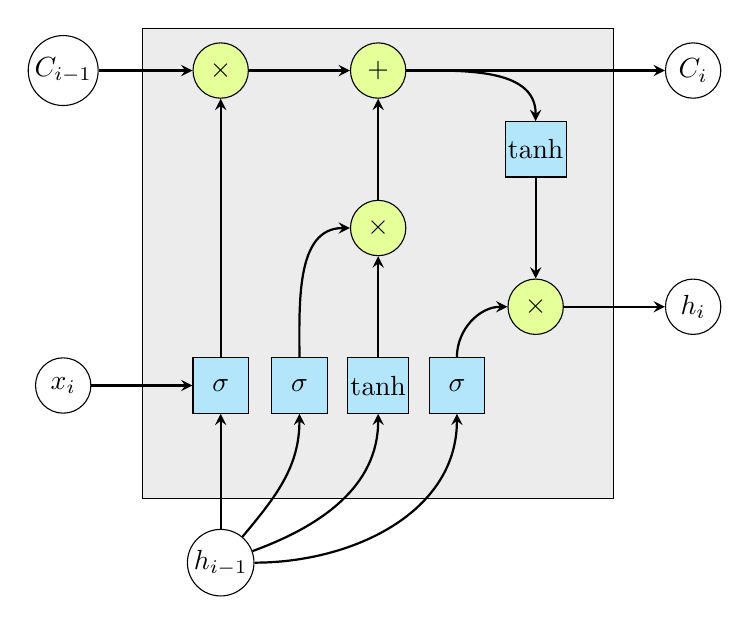
\begin{tikzpicture}
    \node[background_block] (cb) at (0, 1.55){}; 
	\node[block] (s0) at (-2, 0) {$\sigma$};
	\node[block] (s1) at (-1, 0) {$\sigma$};
	\node[block] (s2) at (0, 0) {tanh};
	\node[block] (s3) at (1, 0) {$\sigma$};
    \node[block] (s4) at (2,3) {tanh};

    \node[circle_node] (cn0) at (-2,4) {$\times$};
    \node[circle_node] (cn1) at (0,2) {$\times$};
    \node[circle_node] (cn2) at (0,4) {$+$};
    \node[circle_node] (cn3) at (2,1) {$\times$};

	\draw[stateTransition] (s0) to[out=90,in=270] node [midway, sloped, above] {} (cn0);
	\draw[stateTransition] (s1) to[out=90,in=180] node [midway, sloped, above] {} (cn1);
	\draw[stateTransition] (s2) to[out=90,in=270] node [midway, sloped, above] {} (cn1);
	\draw[stateTransition] (cn1) to[out=90,in=270] node [midway, sloped, above] {} (cn2);
	\draw[stateTransition] (cn0) to[out=0,in=180] node [midway, sloped, above] {} (cn2);
	\draw[stateTransition] (s3) to[out=90,in=180] node [midway, sloped, above] {} (cn3);
	\draw[stateTransition] (cn2) to[out=0,in=90] node [midway, sloped, above] {} (s4);
	\draw[stateTransition] (s4) to[out=270,in=90] node [midway, sloped, above] {} (cn3);

    \node[clearNode] (i0) at (-4, 4) {$\mathpzc{C}_{i-1}$};
    \node[clearNode] (i1) at (4, 4) {$\mathpzc{C}_{i}$};
    \node[clearNode] (i2) at (4, 1) {$h_i$};
    \node[clearNode] (i3) at (-4, 0) {$x_i$};
    \node[clearNode] (i4) at (-2, -2.25) {$h_{i-1}$};

	\draw[stateTransition] (i0) to[out=0,in=180] node [midway, sloped, above] {} (cn0);
	\draw[stateTransition] (cn2) to[out=0,in=180] node [midway, sloped, above] {} (i1);
	\draw[stateTransition] (cn3) to[out=0,in=180] node [midway, sloped, above] {} (i2);
	\draw[stateTransition] (i4) to[out=90,in=270] node [midway, sloped, above] {} (s0);
	\draw[stateTransition] (i3) to[out=0,in=180,  looseness=1] node [midway, sloped, above] {} (s0);
	\draw[stateTransition] (i4) to[out=50,in=270, looseness=1] node [midway, sloped, above] {} (s1);
	\draw[stateTransition] (i4) to[out=20,in=270, looseness=1] node [midway, sloped, above] {} (s2);
	\draw[stateTransition] (i4) to[out=0,in=270, looseness=1] node [midway, sloped, above] {} (s3);

\end{tikzpicture}

\end{document}